\documentclass[oneside, 11pt]{article}

\usepackage[T1]{fontenc}
\usepackage[utf8]{inputenc}
\usepackage[dutch]{babel}

\usepackage{fouriernc}
\usepackage[detect-all, load-configurations=binary,
            separate-uncertainty=true, per-mode=symbol,
            retain-explicit-plus, range-phrase={ tot }]{siunitx}

\usepackage{setspace}
\setstretch{1.2}

\setlength{\parskip}{\smallskipamount}
\setlength{\parindent}{0pt}

\usepackage{geometry}
\geometry{marginparwidth=0.5cm, verbose, a4paper, tmargin=3cm, bmargin=3cm, lmargin=2cm, rmargin=2cm}

\usepackage{float}

\usepackage[fleqn]{amsmath}
\numberwithin{equation}{section}
\numberwithin{figure}{section}

\usepackage{graphicx}
\graphicspath{{Figures/}}
\usepackage{subfig}

\usepackage{tikz}
\usetikzlibrary{plotmarks}

\usepackage{fancyhdr}
\pagestyle{fancy}
\fancyhf{}
\rhead{\thepage}
\renewcommand{\footrulewidth}{0pt}
\renewcommand{\headrulewidth}{0pt}

\usepackage{relsize}
\usepackage{xspace}
\usepackage{url}

\newcommand{\figref}[1]{Figuur~\ref{#1}}

\newcommand{\hisparc}{\textsmaller{HiSPARC}\xspace}
\newcommand{\kascade}{\textsmaller{KASCADE}\xspace}
\newcommand{\sapphire}{\textsmaller{SAPPHiRE}\xspace}
\newcommand{\jsparc}{\textsmaller{jSparc}\xspace}
\newcommand{\hdf}{\textsmaller{HDF5}\xspace}
\newcommand{\aires}{\textsmaller{AIRES}\xspace}
\newcommand{\csv}{\textsmaller{CSV}\xspace}
\newcommand{\python}{\textsmaller{PYTHON}\xspace}
\newcommand{\corsika}{\textsmaller{CORSIKA}\xspace}
\newcommand{\labview}{\textsmaller{LabVIEW}\xspace}
\newcommand{\daq}{\textsmaller{DAQ}\xspace}
\newcommand{\adc}{\textsmaller{ADC}\xspace}
\newcommand{\adcs}{\textsmaller{ADC}s\xspace}
\newcommand{\Adcs}{A\textsmaller{DC}s\xspace}
\newcommand{\hi}{\textsc{h i}\xspace}
\newcommand{\hii}{\textsc{h ii}\xspace}
\newcommand{\mip}{\textsmaller{MIP}\xspace}
\newcommand{\hisparcii}{\textsmaller{HiSPARC II}\xspace}
\newcommand{\hisparciii}{\textsmaller{HiSPARC III}\xspace}
\newcommand{\pmt}{\textsmaller{PMT}\xspace}
\newcommand{\pmts}{\textsmaller{PMT}s\xspace}

\DeclareSIUnit{\electronvolt}{\ensuremath{\mathrm{e\!\!\:V}}}

\DeclareSIUnit{\unitsigma}{\ensuremath{\sigma}}
\DeclareSIUnit{\mip}{\textsmaller{MIP}}
\DeclareSIUnit{\adc}{\textsmaller{ADC}}

\DeclareSIUnit{\gauss}{G}
\DeclareSIUnit{\parsec}{pc}
\DeclareSIUnit{\year}{yr}



\title{Uitleg HiSPARC}
\author{C.G. van Veen}
\docalgemeen{3}{HT}
\version{1.3}

\begin{document}

\maketitle

\section{Inleiding}

De aarde wordt continu gebombardeerd door kosmische straling.
\footnote{Bij dit blad is ook een powerpoint beschikbaar, te vinden op:
docs.hisparc.nl/ bij teaching material.}
Dat zijn deeltjes die uit het heelal vandaan komen zoals protonen, ijzerkernen en
koolstofkernen etc. Deze primaire deeltjes hebben energieën variërend
van \SIrange{e2}{e20}{\electronvolt}. De deeltjes met lagere
waarden voor energie zijn bijvoorbeeld deeltjes uitgezonden door de zon.
De deeltjes met hogere energiewaarden (\SI{>e17}{\electronvolt}) hebben
een energie die we op aarde in versnellers niet kunnen bereiken. Het
noorderlicht ontstaat door deeltjes met een energie in de orde van een
keV, die op stikstof- en zuurstof moleculen botsen. Als primaire
deeltjes energieën hebben in de orde van \SIrange{e14}{e20}
{\electronvolt} en op atomen in de atmosfeer botsen ontstaat een lawine
van allerlei secundaire deeltjes, zie \figref{fig:main_cosmicray_shower}, dat
een Extended Air Shower (EAS) wordt genoemd. Deze EAS reikt afhankelijk
van de energie van het primaire deeltje en de hoogte van de eerste
botsing tot het aardoppervlak. Victor Hess was de eerste die deze EAS of
kosmische showers daadwerkelijk gemeten heeft tijdens diverse metingen
met een luchtballon in 1912. Hess merkte dat de intensiteit van de
achtergrond straling hoger werd naarmate hij hoger in de atmosfeer kwam.
Men dacht toen straling voornamelijk uit de aarde afkomstig moest zijn
en de intensiteit dus zou moeten afnemen naar mate je verder van de
aarde af kwam. Tegenwoordig wordt er veel onderzoek verricht aan
kosmische straling en EAS, door onder andere de volgende
onderzoeksgroepen: KASCADE, AUGER. In Nederland is dit op scholen
mogelijk met HiSPARC.

\begin{figure}
    \centering
    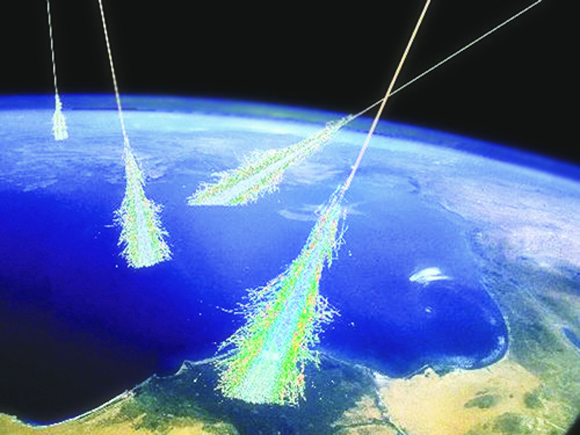
\includegraphics[width=\textwidth]{main_cosmicray_shower}
    \caption{visualisatie van kosmische straling
             (bron: S. Swordy, Universiteit van Chicago).}
    \label{fig:main_cosmicray_shower}
\end{figure}

\section{\hisparc}

Het Nederlandse project \hisparc is een samenwerking van middelbare scholen en universiteiten.
Op deze scholen en universiteiten zijn detectie stations geplaatst waarmee we EAS kunnen
meten en analyseren. Leraren en leerlingen installeren, beheren en onderhouden de stations,
en houden de kwaliteit van de ermee verkregen meetgegevens in de gaten.
Zo worden EAS in een groot oppervlak gemeten en worden middelbare
scholieren betrokken bij wetenschappelijk onderzoek ondersteund door
universiteiten. Het doel van HiSPARC is om met behulp van de stations op
scholen onderzoek te doen aan deze kosmische showers. Onderzoeksvragen
met betrekking tot kosmische straling zijn, waar deze vandaan komen en
hoe ze ontstaan. De energie en richting zijn af te leiden uit de grootte
van de EAS en de tijdsverschillen in de detectoren. Waar kosmische
straling vandaan komt is gedeeltelijk bekend. Laag-energetische deeltjes
komen van de zon (de zonnewind) en van sterren uit ons melkwegstelsel.
Deeltjes met energieën tot ongeveer \SI{e16}{\electronvolt} zijn
afkomstig van supernova's. Deeltjes met nog meer energie kunnen aan
magneetvelden van sterrenstelsels ontsnappen en zijn waarschijnlijk
buiten ons melkwegstelsel ontstaan. Hierbij denkt men aan een oorsprong
van primaire deeltjes uit Gamma-Ray Bursts (GRB), aan actieve kernen van
ver weg gelegen sterrenstelsels, en aan andere verschijnselen die met
zeer energetische plasmajets gepaard gaan. Kosmische straling kan
afkomstig zijn van zwarte gaten en actieve sterrenstelsels.

\section{Aantal kosmische showers}

Het aantal kosmische showers wat gemeten wordt, hangt sterk af van de
energie van het primaire deeltje. Primaire deeltjes met een 10 maal zo
hoge energie komen globaal 1000 maal zo weinig voor. In
\figref{fig:swordy_blois} zie je het diagram (op een dubbel
logaritmische schaal) wat het overzicht geeft tussen de flux (aantal
showers per tijdseenheid per oppervlak) tegen de energie van het
primaire deeltje. Hierin is te zien dat het aantal deeltjes met een
energie van \SI{e19}{\electronvolt} één keer per jaar op een oppervlak
van \SI{1}{\square\kilo\meter} komt, door één \si{\square\meter} gaat
per seconde gemiddeld een deeltjes met een energie van
\SI{e11}{\electronvolt}. Duidelijk is te zien dat de grafiek tussen
\SIrange{e20}{e21}{\electronvolt} ogenschijnlijk ophoudt. Deze grens
wordt de ‘GZK cut-off’ genoemd. (Greisen–Zatsepin–Kuzmin limiet). Men
vermoedt dat de ‘GZK’ bovengrens vormt voor de energie van kosmische
straling. Zeker weten doen we dat niet omdat die energieën heel zeldzaam
zijn.

\begin{figure}
    \centering
    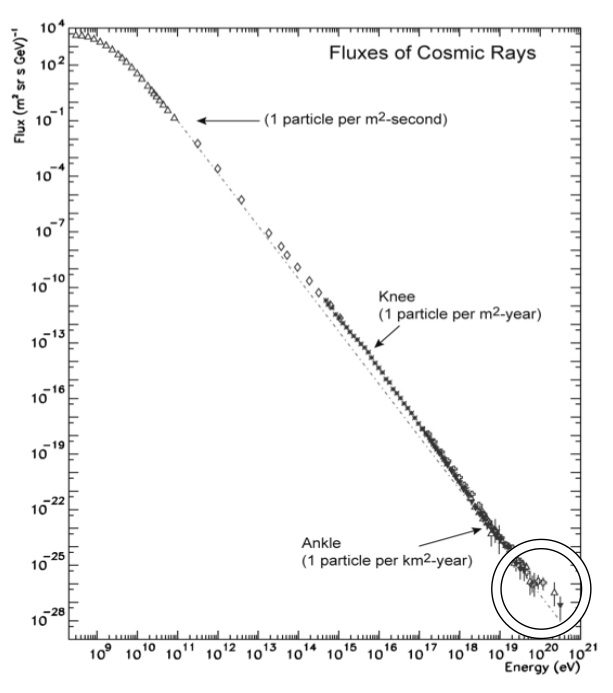
\includegraphics[width=\textwidth]{swordy_blois}
    \caption{Flux als functie van de energie van kosmische straling. Tussen
             \SIlist{1e11;1e15}{\electronvolt} meten we bijna geen flux omdat
             showers die ontstaan door deeltjes met deze energieën de grond
             niet bereiken. (bron: S. Swordy, Universiteit van Chicago)}
    \label{fig:swordy_blois}
\end{figure}

Je kunt het onderzoek van \hisparc vergelijken met onderzoek van
sterrenkundigen. Sterrenkundigen bestuderen sterren met behulp van het
licht wat sterren en hemelobjecten uitzenden of terugkaatsen. De
informatie die zij vinden en gebruiken zit ‘opgesloten’ in het licht wat
opgevangen wordt. De mensen die de data van \hisparc onderzoeken,
bestuderen de kosmische showers aan de hand van de detectoren die op de
scholen en universiteiten staan. Zij meten de hoeveelheid deeltjes per
oppervlakte eenheid en kijken naar tijdsverschillen tussen aankomst van
de deeltjes in de detectoren, daarmee kunnen ze informatie over de EAS
herleiden. De \hisparc stations meten de deeltjes van de EAS die
het aardoppervlak bereiken en zijn via een netwerk verbonden met het
Nikhef en de Universiteit van Nijmegen. De \hisparc detectoren kunnen
de fotonen, muonen en elektronen meten die in zo’n EAS voorkomen, zie \figref{fig:shower}.
Een station bestaat uit twee of vier detectoren, die ieder
een eigen signaal bij een detectie van een EAS geven; de pulshoogte. Is
het signaal hoog genoeg en meten twee of meer detectoren binnen een kort
tijdspanne een signaal, dan slaat het meetstation dit signaal als een
event op in de database. Het registreren van een signaal in een detector wordt
uitgebreid uitgelegd in het document "Inregelen PMT's".
Web-adres: \url{https://docs.hisparc.nl/infopakket//}.
Per uur worden typisch zo’n 2000 tot 3000
events geregistreerd per station. Als meerdere detectoren of stations
binnen een bepaalde tijd deeltjes detecteren dan spreken we van een
coïncidentie. Bij een coïncidentie behoren dus alle metingen op dat
moment bij één EAS.

\begin{figure}
    \centering
    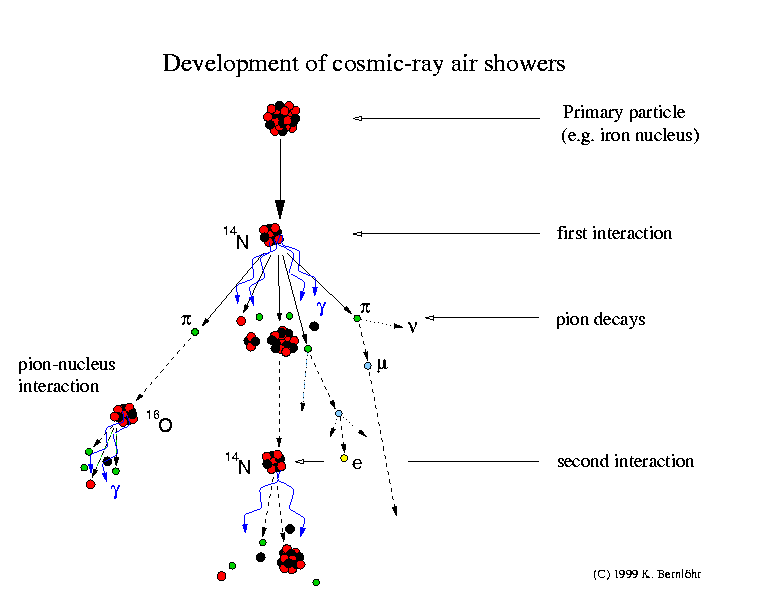
\includegraphics[width=0.8\textwidth]{shower}
    \caption{Als een primair deeltje op de atmosfeer komt, kan er een botsing
             plaatsvinden met een atoom, door die botsing ontstaan er andere
             elementaire deeltjes en fotonen. copyright: Konrad Bernlöher}
    \label{fig:shower}
\end{figure}

\section{Reconstructies uit de showers}

Momenteel richt het \hisparc onderzoek zich op het reconstrueren
van de richting  en energie van gedetecteerde showers. De benodigde data kun je opvragen
van \hisparc netwerk, via de volgende website,
\url{https://data.hisparc.nl/media/jsparc/data_retrieval.html} Hoe de
data retrieval tool werkt en hoe je er snelle analyses mee kunt doen en
correlaties tussen verschillende grootheden kunt zoeken wordt uitgelegd
in het infopakket van \hisparc, in het bestand `Data-retrieval' op het
webadres van infopakket:
\url{https://docs.hisparc.nl/infopakket//}

Als er data wordt gedownload via de data retrieval zie je dat er een aantal
gegevens worden gemeten met de stations \figref{fig:data_retrieval}. Voor de
reconstructie van de richting waaruit de kosmische shower komt en de energie
van het deeltje zijn een aantal kolommen van belang, zoals de Arrival time,
Pulseheight, Pulseintegral en Number of MIP's \footnote{Meer over de terminologie
van kosmische showers vind je in het bestand `Terminologie' van het infopakket}.

De deeltjes, die geproduceerd worden in een kosmische shower, invallen op de
detectoren kan uit de gemeten puls informatie worden gehaald, die leidt tot de
kolommen: Arrival time, Pulseheight, Pulseintegral, Number of MIP's.
Met de informatie in deze kolommen wordt de richting en energie van de kosmische
showers zo nauwkeurig mogelijk gereconstrueerd. In \figref{fig:traces} zie je
dat elk meetstation per gemeten event per detector een signaal geeft, maar
dat ze niet even hoog zijn, m.a.w. een lagere pulshoogte betekent dat er
minder deeltjes geregistreerd
zijn.

\begin{figure}
    \centering
    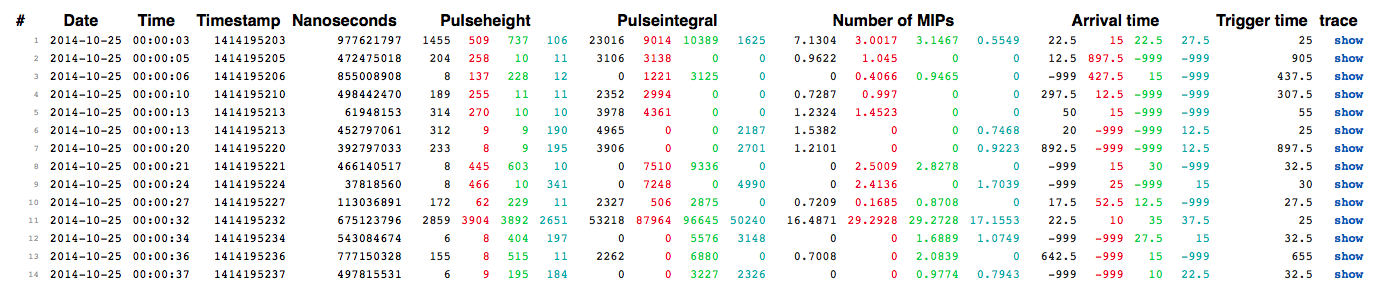
\includegraphics[width=\textwidth]{data_retrieval}
    \caption{Als met de (online) data-retrieval tool, data wordt gedownload dan zijn
    er een aantal belangrijke kolommen voor reconstructie te zien, zoals Arrival time,
    Pulseheight, Pulseintegral en Number of MIP's.}
    \label{fig:data_retrieval}
\end{figure}

\subsection{Reconstructie van shower richting}

Je ziet in \figref{fig:Arrivaltime_pulse}, dat de detectoren op
verschillende tijdstippen hun puls beginnen. De zwarte grafiek in
\figref{fig:Arrivaltime_pulse} heeft de laatste Arrival time. De Arrival
time wordt bepaald zoals in \figref{fig:Arrivaltime_pulse} wordt getoond.
De flank van de pulse moet over een bepaalde drempelwaarde heen gaan,
dan wordt die tijd waarop dat gebeurd opgeslagen als Arrival time voor
die puls. Nu we voor één event de Arrival times hebben bepaald kunnen we
met goniometrische beschouwingen, de richting vanwaar deze shower kwam, uitrekenen.
Hoe dit precies in zijn werk gaat is na te lezen in het infopakket van
\hisparc, in het bestand `richting reconstructie' op het webadres:
\url{https://docs.hisparc.nl/infopakket/} Als leerlingen een richtingreconstructie willen doen
dan kunnen ze dat oefenen met het werkblad `richting primair deeltje' van het RouteNet
materiaal op de website: \url{https://docs.hisparc.nl/routenet/routenet.html}.

\begin{figure}
    \centering
    \documentclass[oneside, 11pt]{article}

\usepackage[T1]{fontenc}
\usepackage[utf8]{inputenc}
\usepackage[dutch]{babel}

\usepackage{fouriernc}
\usepackage[detect-all, load-configurations=binary,
            separate-uncertainty=true, per-mode=symbol,
            retain-explicit-plus, range-phrase={ tot }]{siunitx}

\usepackage{setspace}
\setstretch{1.2}

\setlength{\parskip}{\smallskipamount}
\setlength{\parindent}{0pt}

\usepackage{geometry}
\geometry{marginparwidth=0.5cm, verbose, a4paper, tmargin=3cm, bmargin=3cm, lmargin=2cm, rmargin=2cm}

\usepackage{float}

\usepackage[fleqn]{amsmath}
\numberwithin{equation}{section}
\numberwithin{figure}{section}

\usepackage{graphicx}
\graphicspath{{Figures/}}
\usepackage{subfig}

\usepackage{tikz}
\usetikzlibrary{plotmarks}

\usepackage{fancyhdr}
\pagestyle{fancy}
\fancyhf{}
\rhead{\thepage}
\renewcommand{\footrulewidth}{0pt}
\renewcommand{\headrulewidth}{0pt}

\usepackage{relsize}
\usepackage{xspace}
\usepackage{url}

\newcommand{\figref}[1]{Figuur~\ref{#1}}

\newcommand{\hisparc}{\textsmaller{HiSPARC}\xspace}
\newcommand{\kascade}{\textsmaller{KASCADE}\xspace}
\newcommand{\sapphire}{\textsmaller{SAPPHiRE}\xspace}
\newcommand{\jsparc}{\textsmaller{jSparc}\xspace}
\newcommand{\hdf}{\textsmaller{HDF5}\xspace}
\newcommand{\aires}{\textsmaller{AIRES}\xspace}
\newcommand{\csv}{\textsmaller{CSV}\xspace}
\newcommand{\python}{\textsmaller{PYTHON}\xspace}
\newcommand{\corsika}{\textsmaller{CORSIKA}\xspace}
\newcommand{\labview}{\textsmaller{LabVIEW}\xspace}
\newcommand{\daq}{\textsmaller{DAQ}\xspace}
\newcommand{\adc}{\textsmaller{ADC}\xspace}
\newcommand{\adcs}{\textsmaller{ADC}s\xspace}
\newcommand{\Adcs}{A\textsmaller{DC}s\xspace}
\newcommand{\hi}{\textsc{h i}\xspace}
\newcommand{\hii}{\textsc{h ii}\xspace}
\newcommand{\mip}{\textsmaller{MIP}\xspace}
\newcommand{\hisparcii}{\textsmaller{HiSPARC II}\xspace}
\newcommand{\hisparciii}{\textsmaller{HiSPARC III}\xspace}
\newcommand{\pmt}{\textsmaller{PMT}\xspace}
\newcommand{\pmts}{\textsmaller{PMT}s\xspace}

\DeclareSIUnit{\electronvolt}{\ensuremath{\mathrm{e\!\!\:V}}}

\DeclareSIUnit{\unitsigma}{\ensuremath{\sigma}}
\DeclareSIUnit{\mip}{\textsmaller{MIP}}
\DeclareSIUnit{\adc}{\textsmaller{ADC}}

\DeclareSIUnit{\gauss}{G}
\DeclareSIUnit{\parsec}{pc}
\DeclareSIUnit{\year}{yr}



\title{Pulshoogte en pulsintegraal}
\author{N.G. Schultheiss}
\docwerkblad{2}{PH}
\version{1.0}

\begin{document}

\maketitle

\section{Inleiding}

Elke detector van een \hisparc-station is uitgerust met een
foto-versterker buis (PhotoMultiplier Tube: \pmt). Als er geen deeltjes
door de detector schieten, treedt er geen fluorescentie in de detector
op en ontstaat er geen licht. In dit geval geeft de PMT-buis een
elektrisch signaal van \SI{0}{\milli\volt} aan de \hisparc unit. Als er
wel deeltjes door de detector schieten, treedt er fluorescentie in de
detector op en ontstaat er licht. Dan geeft de PMT-buis een elektrisch
signaal af waarvan het aantal mV afhangt van het aantal deeltjes dat
door de detector is gegaan. In de \hisparc unit wordt het analoge
signaal door middel van een Analoog Digitaal Converter (\adc) omgezet in
een digitaal signaal. De grootte van dit signaal wordt uitgedrukt in
\adcs, de \adc count (een getal zonder eenheid).

Als er een detectorsignaal gemeten wordt, wordt een reeks van deze \adcs
in de \hisparc unit opgeslagen. Als er tegelijkertijd een tweede reeks,
van een andere detector, wordt opgeslagen, worden alle reeksen \adcs van
de \hisparc unit naar de \hisparc server gezonden. Met dergelijke reeks
kan een diagram van het verloop van het signaal tegen de tijd worden
gemaakt. In deze diagrammen zijn van het negatieve maximale signaal de
pulshoogte en het oppervlak, de pulsintegraal, te bepalen. Gedurende de
dag worden alle pulshoogten en pulsintegralen van een station verzameld.
Pulshoogte en pulsintegraal histogrammen zijn op te vragen op:
\url{http://data.hisparc.nl/} door op de stationsnaam te klikken.
Rechtsboven beide histogrammen is een link waarmee de gegevens in een
spreadsheet, zoals Excel, te laden zijn.


\section{De pulsvorm}


\subsection{Pulsen ophalen uit de \hisparc data opslag}

\begin{figure}[ht]
    \centering
    \subfloat{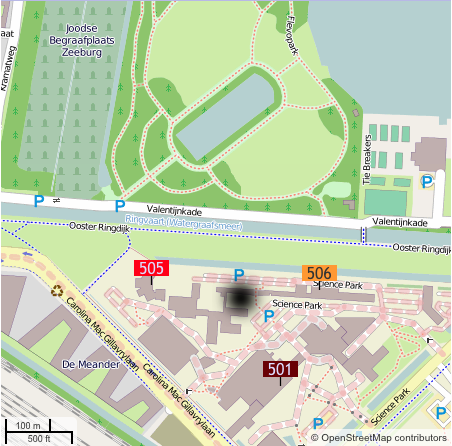
\includegraphics[scale=0.33]{kaart}}
    \subfloat{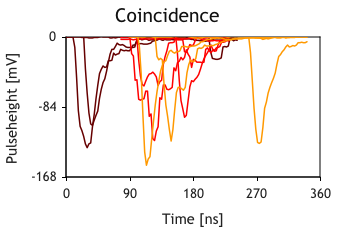
\includegraphics[scale=0.65]{Coincidence}}
    \caption{De plattegrond met de locaties van de meetstations
             en de gemeten pulsen per station.}
    \label{fig:coincidence}
\end{figure}

In de praktijk kunnen we een set pulsen voor een willekeurige
gebeurtenis ophalen met \jsparc%
\footnote{Het interactieve practicum \jsparc kan in de les na aanvraag
van een sessie worden gebruikt, het is ook mogelijk om een willekeurige
set pulsen op te halen op:
\url{http://data.hisparc.nl/media/jsparc/jsparc.html}.%
}. In deze module gaan we uit van de set pulsen die met de stations
uit \figref{fig:coincidence} zijn gemeten.

Op de kaart zijn drie meetstations te zien, een bruin, een rood en een
oranje station%
\footnote{De kleuren van de stations volgen de definitie van de
kleurcode van weerstandjes: bruin: 1, rood: 2, oranje: 3, geel: 4,
groen: 5, blauw: 6, violet: 7, etc. %
}. We zien dat alle stations meerdere pulsen hebben gegeven, dit komt
omdat een station uit meerdere detectoren bestaat. De hoogtes van de
pulsen zijn vergelijkbaar, bijgevolg is het midden van de air-shower
(zwarte vlek in \figref{fig:coincidence}) even ver van alle stations.


\subsection{Eenvoudige pulsvormen}

Het is mogelijk om de diagrammen per detector van een enkel station
te bekijken. In \figref{fig:Eenvoudige-pulsen} zijn de signalen
van vier detectoren van Station 506 te zien. De zwarte puls van detector
1 heeft een vrij steile voorflank. Het verloop van de achterflank
lijkt een halfwaardetijd te hebben (deze loopt exponentieel op). Bij
de blauwe grafiek van detector 4 is iets soortgelijks aan de hand.
Een deeltje lijkt dus herkend te worden aan een steile dalende flank
die wordt gevolgd door een exponentieel oplopende achterflank.

\begin{figure}[ht]
    \centering
    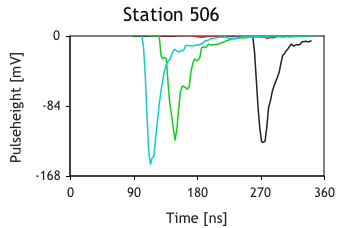
\includegraphics[scale=0.65]{Traces506}
    \caption{Eenvoudige pulsen}
    \label{fig:Eenvoudige-pulsen}
\end{figure}


\begin{minipage}[t]{1\columnwidth}%

\paragraph{Opdracht 1:}

De groene grafiek van detector 3 in \figref{fig:Eenvoudige-pulsen}
heeft een minder vloeiend verloop. Stel een hypothese op waarmee dit
minder vloeiende verloop kan worden verklaard.

\begin{center}
    \rule{\textwidth}{0.3mm}\\
    \rule{\textwidth}{0.3mm}\\
    \rule{\textwidth}{0.3mm}\\
    \rule{\textwidth}{0.3mm}\\
\end{center}
\end{minipage}

\bigskip{}


Meestal zien de grafieken er niet zo mooi uit als in
\figref{fig:Eenvoudige-pulsen}. In \figref{fig:Iets-complexere-pulsen}
zijn andere pulsen van detector 1 en 4 van Station 501 te zien
(respectievelijk zwart en blauw).

\begin{figure}[ht]
    \centering
    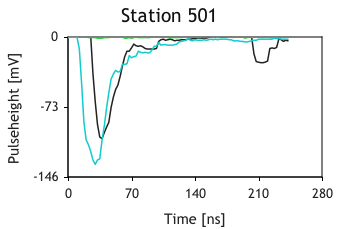
\includegraphics[scale=0.65]{Traces501}
    \caption{Iets complexere pulsen}
    \label{fig:Iets-complexere-pulsen}
\end{figure}


\begin{minipage}[t]{1\columnwidth}%

\paragraph{Opdracht 2:}

Geef een verklaring voor het verloop van de grafiek van detector
1 in \figref{fig:Iets-complexere-pulsen}.

\begin{center}
    \rule{\textwidth}{0.3mm}\\
    \rule{\textwidth}{0.3mm}\\
    \rule{\textwidth}{0.3mm}\\
    \rule{\textwidth}{0.3mm}\\
\end{center}
\end{minipage}

\bigskip{}


\begin{minipage}[t]{1\columnwidth}%

\paragraph{Opdracht 3:}

Bereken de afstand tussen de waargenomen deeltjes in de grafiek
van detector 1 (zwart) in \figref{fig:Iets-complexere-pulsen}.

\begin{center}
    \rule{\textwidth}{0.3mm}\\
    \rule{\textwidth}{0.3mm}\\
    \rule{\textwidth}{0.3mm}\\
    \rule{\textwidth}{0.3mm}\\
\end{center}
\end{minipage}


\subsection{Ingewikkelde pulsvormen}

\begin{figure}[ht]
    \centering
    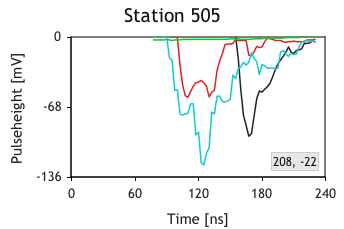
\includegraphics[scale=0.65]{Traces505}
    \caption{Ingewikkelde pulsvormen}
    \label{fig:Ingewikkelde-pulsvormen}
\end{figure}


\bigskip{}

In \figref{fig:Ingewikkelde-pulsvormen} valt het op dat de pulshoogte
van detector 2 (rood) kleiner is dan detector 1 (zwart).

\begin{minipage}[t]{1\columnwidth}%

\paragraph{Opdracht 4:}

Leg met de pulsintegraal (het pulsoppervlak) uit waarom er
waarschijnlijk evenveel deeltjes door detector 1 als door detector
2 zijn gegaan.

\begin{center}
    \rule{\textwidth}{0.3mm}\\
    \rule{\textwidth}{0.3mm}\\
    \rule{\textwidth}{0.3mm}\\
    \rule{\textwidth}{0.3mm}\\
\end{center}
\end{minipage}

\bigskip{}


In \figref{fig:Ingewikkelde-pulsvormen} valt het verder op dat detector
3 (groen) bijna geen puls geeft.

\begin{minipage}[t]{1\columnwidth}%

\paragraph{Opdracht 5:}

Verklaar waarom er binnen een station soms detectoren zijn
die een aantal deeltjes meten terwijl ander detectoren (bijna) niets
meten.

\begin{center}
    \rule{\textwidth}{0.3mm}\\
    \rule{\textwidth}{0.3mm}\\
    \rule{\textwidth}{0.3mm}\\
    \rule{\textwidth}{0.3mm}\\
\end{center}
\end{minipage}
\end{document}

    \caption{Één event gemeten door een station met vier detectoren, elke detector registreert
    een signaal (pulse) die op een eigen tijdstip begint (Arrival Time) en een eigen hoogte heeft
    (Pulse height).}
    \label{fig:traces}
\end{figure}


\begin{figure}
    \centering
    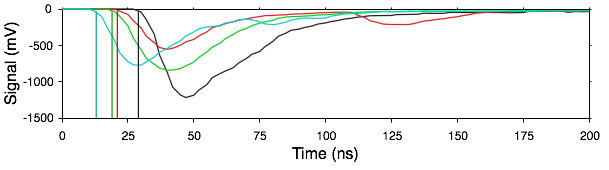
\includegraphics[width=\textwidth]{Arrivaltime_pulse}
    \caption{Als de flank van de pulse over een bepaalde ingestelde
    drempelwaarde gaat, dan wordt dat tijdstip voor die pulse als Arrival
    time opgeslagen. Voor de cyaan kleurige puls komen we zo op een Arrival
    time van 12,5 ns. De Arrival times zijn altijd deelbaar door 2,5 ns, dit
    komt door de ADC converter in het HiSPARC kastje. Meer uitleg hierover
    in het bestand `Uitlijnen van de ADC's' in het \hisparc infopakket.}
    \label{fig:Arrivaltime_pulse}
\end{figure}


\subsection{Reconstructie van energie }

In \figref{fig:pulshoogte} zie je de pulsen van twee detectoren (dit is
dus een twee detector station of een vier detector station, waarbij twee
detectoren `getriggerd' zijn). De maximale waarde van de pulsen is daar
aangegeven met een verticale lijn. De waarde van de potentiaal die bij
dit punt hoort, wordt de `pulseheight' of in het Nederlands `pulshoogte'
genoemd. Als we van alle events, die we op een dag meten met een
station, alle gemeten `pulseheights' plotten in een histogram dan
krijgen we het plaatje zoals te zien is in \figref{fig:MIP_histogram}. Daarin
zetten we het aantal keer dat een bepaalde pulshoogte voorkomt uit tegen
de spanningswaarde van de pulshoogte. De laagste piek van de pulshoogte
komt het vaakst voor en deze waarde geeft dus een maat voor de detectie van
precies één deeltje in een detector. Stel dus dat de waarde van de
pulshoogte \SI{300}{\adc} heel vaak voorkomt op een dag. Dan zul je in het
pulshoogte histogram een piek krijgen bij \SI{300}{\adc}, dit is dan de
waarde die hoort bij één
deeltje wat gedetecteerd is. Meet je bij een ander event in dezelfde detector
een puls van \SI{900}{\adc}, dan zouden er mogelijk 3 deeltjes zijn gedetecteerd
zijn door deze detector. De piek in het pulshoogte histogram noemen we
de MIP (Minimum Ionizing Particle) dat is waarde van de rode lijn in
\figref{fig:MIP_histogram} (in dit geval ongeveer \SI{316}{\adc}).
Deze waarde wordt elke dag per detector elke keer opnieuw bepaalt en gebruikt als ijkmiddel om
het aantal deeltjes te berekenen wat in één event is gedetecteerd. De waarde
van de MIP varieert per detector en per meetperiode, omdat de MIP waarde
afhankelijk is van temperatuur, spanning over de fotobuis, dikte van de
scintillator, montage van de detector en leeftijd van de detector.

\begin{figure}
    \centering
    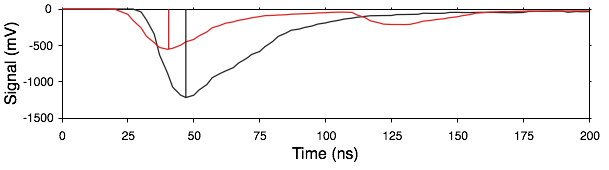
\includegraphics[width=\textwidth]{pulshoogte}
    \caption{Pulseheights van twee detectoren aangegeven.}
    \label{fig:pulshoogte}
\end{figure}

\begin{figure}
    \centering
    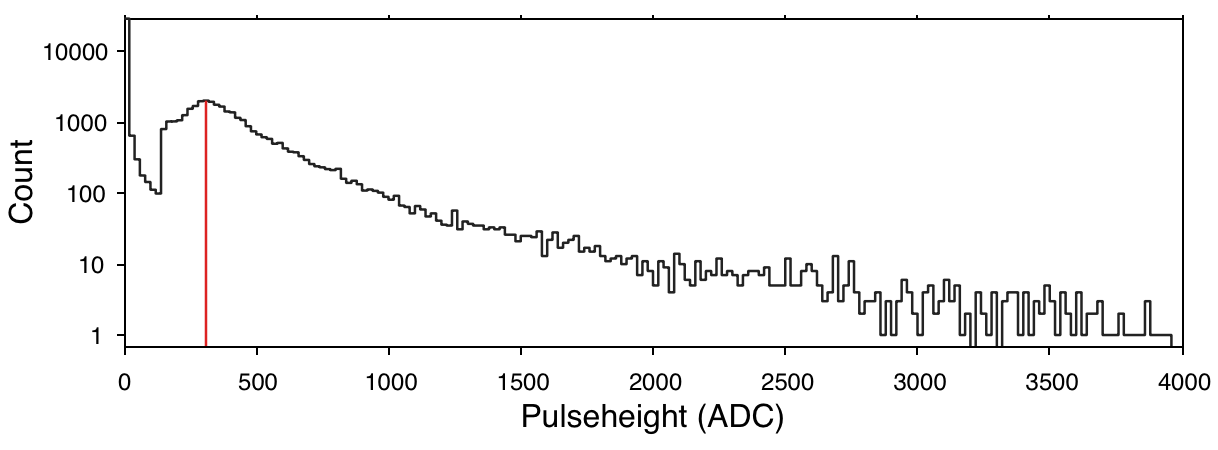
\includegraphics[width=\textwidth]{MIP_histogram}
    \caption{Een pulshoogte histogram, in dit diagram zijn de pulseheights van veel
    gemeten events door één detector uitgezet. De piek is de pulshoogte,
    die hoort bij de detectie van één deeltje. Dit is de MIP piek. In dit geval is
    de MIP \SI{\pm316}{\adc}. De MIP piek wordt gebruikt om de deeltjes
    dichtheid in de detector voor alle geregistreerde events uit te
    rekenen.}
    \label{fig:MIP_histogram}
\end{figure}

Nu we met behulp van de MIP\footnote{Meer over de MIP piek vind je in
het bestand `inregelen PMT's' van het \hisparc infopakket} piek van elke
detector kunnen bepalen wat het aantal deeltjes in een detector per
event is. Als het aantal deeltjes per detector bekend is kunnen we de
energie van het primaire deeltje wat de shower veroorzaakt
reconstrueren. Omdat we denken te weten hoe de shower zich ontwikkelt in de
atmosfeer, kunnen we met onze metingen van het aantal deeltjes op de
grond aan de hand van \eqref{eq:LDF} een energie van het primaire
deeltje reconstrueren.

Als we een coïncidentie hebben, waarbij meerdere stations dus dezelfde
shower gemeten hebben, kunnen we het aantal gemeten deeltjes per
detector plotten zoals in \figref{fig:particle_density}. Om nu achter de
energie van de kosmische shower te komen moeten we de deeltjes dichtheid
fitten aan formule \eqref{eq:LDF}. Waarin Ne het aantal deeltjes is van de
shower (showersize), s de age parameter en r0 is een aangepaste Molière
straal. De waarden van de constanten zijn: $\alpha$ = 1.5, $\beta$ = 3.6, $r_0$ = 40 m
en s = 0.94\footnote{het uitleggen de constantes in de formule is erg
lastig en vereist een gedegen kennis van de wiskundige ontwikkeling van
de showers, maar als de parameter s is 1,  dan is het aantal deeltjes in
de deeltjeslawine maximaal.}.
Als je meer informatie wilt over de ontwikkeling van een shower, kun je
dat lezen in het bestand `cosmic air showers' in het \hisparc infopakket
(lees dan over het Heitler-model).


De deeltjes lawine wordt gemeten op het aardoppervlak. Midden in het
oppervlak dat geraakt wordt, bevindt zich de kern van de deeltjeslawine,
zie \figref{fig:particle_density}. De deeltjesdichtheid is hier het
grootst. Naarmate we verder van de kern komen, daalt de
deeltjesdichtheid. De laterale distributie functie beschrijft de
verdeling van de deeltjes, die op een oppervlak vallen. Als de laterale
distributie functie bekend is, dan kunnen we de plaats van de kern van
de deeltjes lawine bepalen uit minimaal drie metingen van de
deeltjesdichtheid. Het aantal deeltjes in de lawine is daarmee ook te
bepalen, en dit is een maat voor de energie van het primaire deeltjes.


\begin{figure}
    \centering
    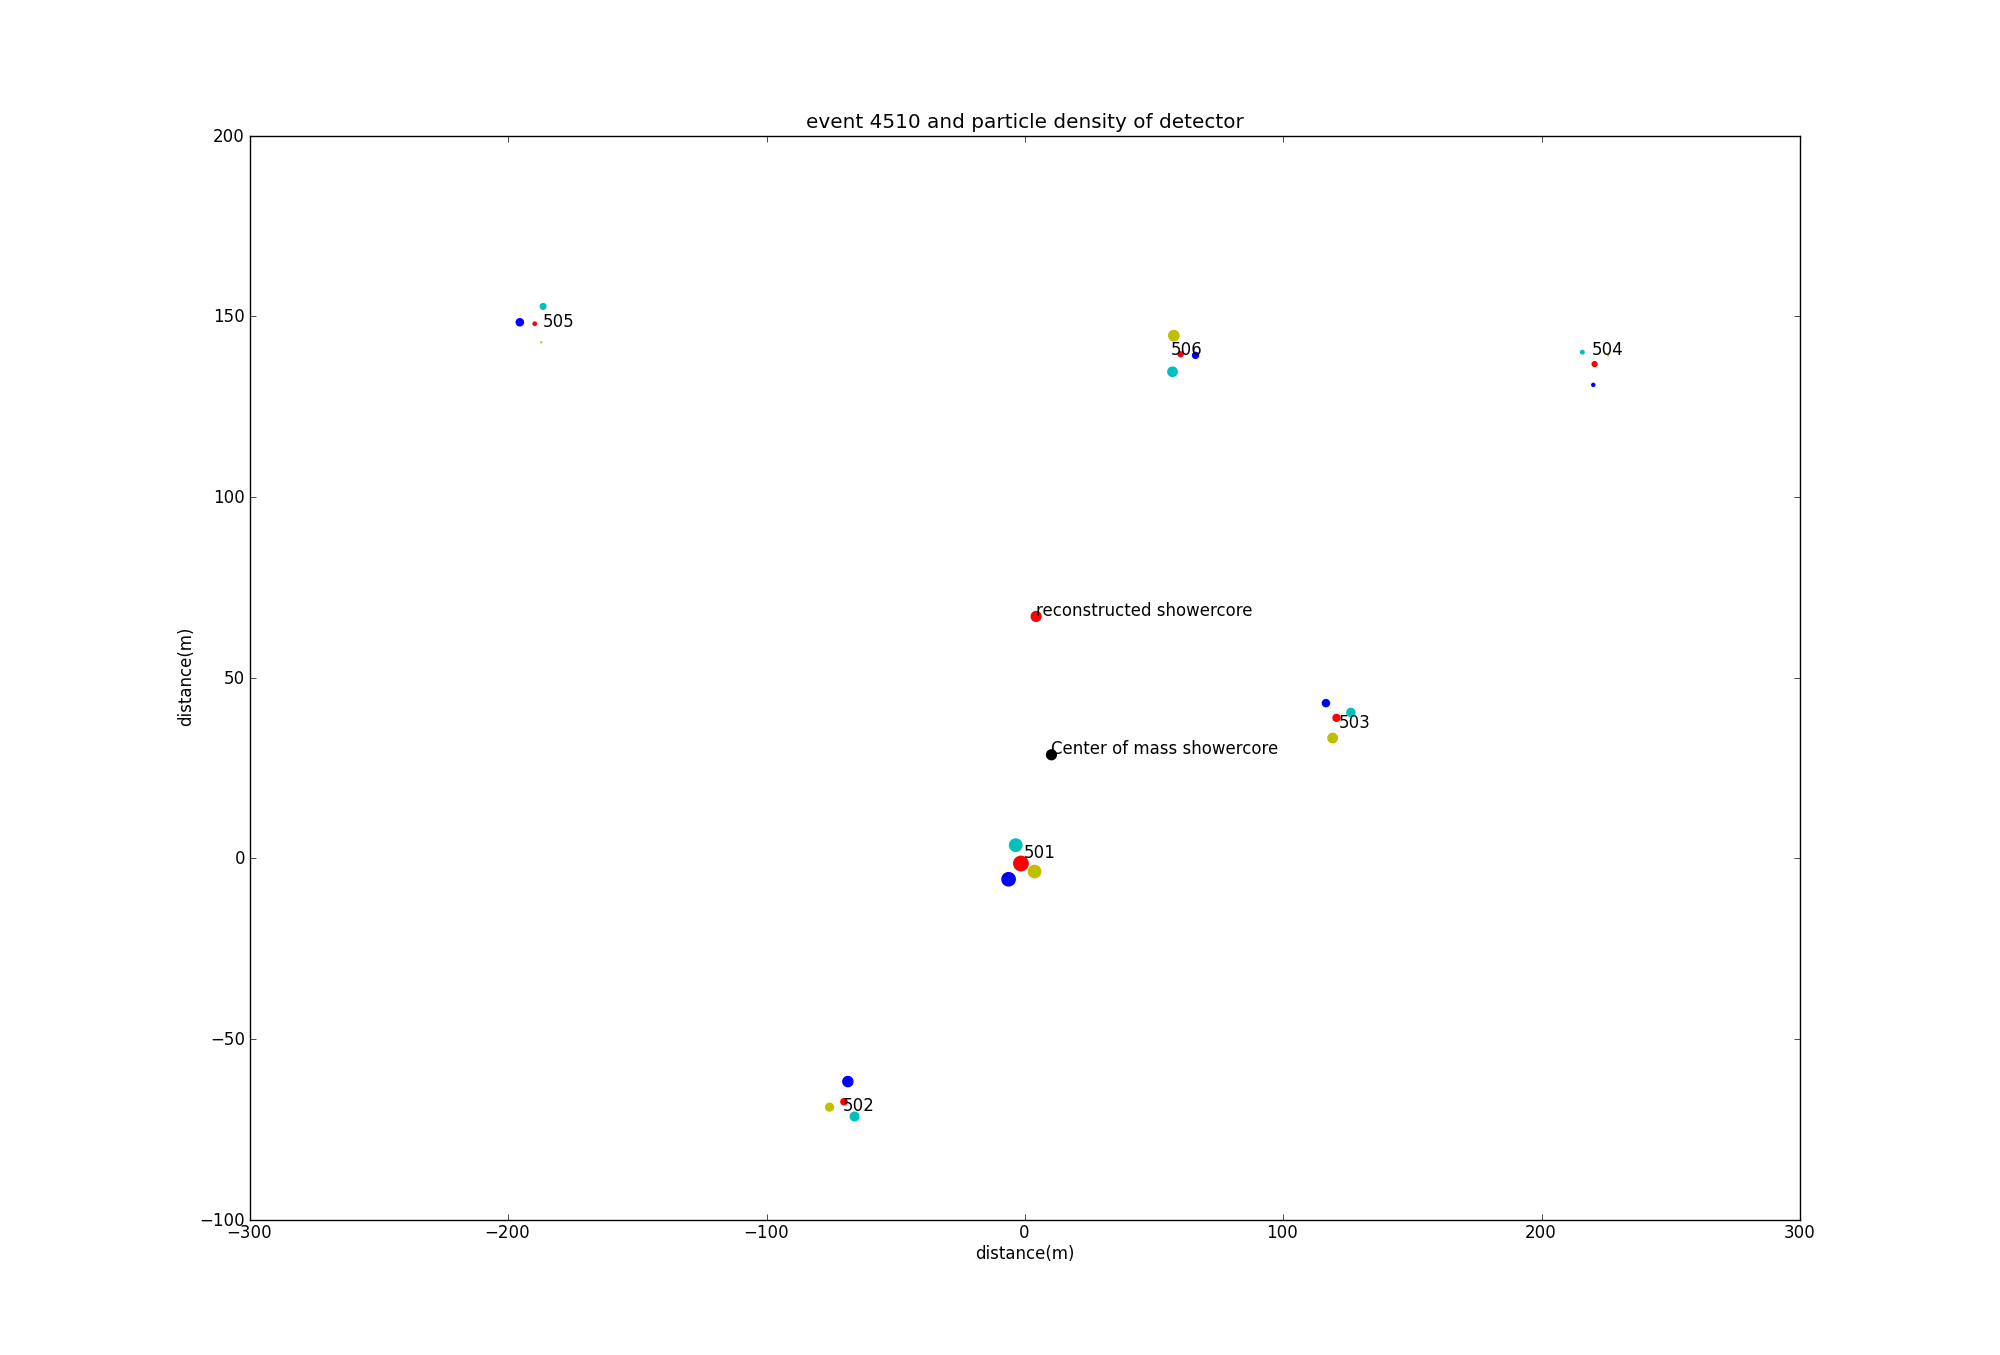
\includegraphics[width=\textwidth]{particle_density}
    \caption{Een geregistreerd event. De nummers van de stations van
    het Sciencepark cluster zijn aangegeven. Van elk station is de
    deeltjesdichtheid van de detectoren weergegeven door de grootte van de
    cirkels. Een grote cirkel komt dus overeen met een grote
    deeltjesdichtheid per detector. Als startwaarde voor de fit aan een
    LDF functie om de positie van een showercore te vinden, kan de
    ‘center of mass’ methode gebruikt worden. Deze methode berekent het
    gewogen gemiddelde van de gemeten deeltjesdichtheid en de afstand
    tot de stations. In dit figuur is ook een gereconstrueerde
    showercore te zien.}
    \label{fig:particle_density}
\end{figure}

\begin{equation}
\rho(r) = N_e \cdot \hat{c}(s) \cdot \left(\frac{r}{r_0}\right)^{s-\alpha} \cdot \left(1 + \frac{r}{r_0}\right)^{s-\beta}
\label{eq:LDF}
\end{equation}

met

\begin{equation}
\hat{c}(s) = \frac{\Gamma(\beta-s)}{2\pi r_0^2 \, \Gamma(s-\alpha+2) \, \Gamma(\alpha+\beta-2s-2)}
\label{eq:gamma}
\end{equation}

waarin $\Gamma$ de gamma functie is.

\begin{figure}
    \centering
    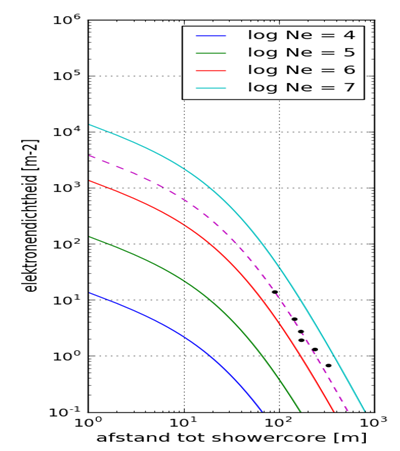
\includegraphics[scale=0.8]{LDF_fit}
    \caption{Een event is gefit aan de LDF \eqref{eq:LDF}. De lijnen geven
    LDF’s van respectievelijk showergrootten van \numrange{e4}{e7} aan. Het
    gereconstrueerde event (stippellijn) van 6 stations (gemiddelde deeltjesdichtheid
    per station) heeft een showersize tussen \num{e6} en \num{e7} deeltjes.}
    \label{fig:LDF_fit}
\end{figure}

\end{document}
